%% "Plantilla para elaborar presentaciones con LaTeX Beamer”%%
\documentclass[11pt,xcolor=pdftex,dvinames,table]{beamer}
\usepackage[utf8]{inputenc}
\usepackage[spanish]{babel}
\usepackage{amsmath}
\usepackage{soul}
\usepackage{color}
\usepackage{amsfonts}
\usepackage{amssymb}
\usepackage{graphicx}
\usepackage{lipsum}
\usepackage{ragged2e}
\usepackage{hyperref}
\usepackage{float}
\usepackage{url} 
\usepackage{verbatim}
\usetheme{PaloAlto}

\author[TL62\_VJQD]{Verónica Jackeline Quiros Díaz}
\title[Planetas]{Sistema Solar}
\date{20 de Agosto de 2020} 
\subtitle{Presentación básica en \LaTeX}
\begin{document}
	\begin{frame}
		\maketitle
	\end{frame}
    \begin{frame}{Índice}
		\tableofcontents
	\end{frame}
    \section{Sistema Solar}
    \justifying
		\begin{frame}{Sistema Solar}
    		El sistema solar cuenta con 8 planetas y 5 planetas enanos reconocidos. Han sido objeto de estudio desde hace cientos y cientos de años, pero, aún así, siguen quedando muchos enigmas por resolver y, año tras año, seguimos recibiendo nueva información sobre ellos.
    		\vfill
    		\centering
    		\rowcolors{1}{green!30}{green!15}
            \begin{tabular}{ll}\hline
            \textbf{Término}& \textbf{Descripción}\\
            Sistema Solar & Compuesto por el Sol y 8 planetas\\
            \end{tabular}
		\end{frame}
	\subsection{Planetas}	
	    \begin{frame}{Planetas}
			\justifying
			Estas son algunas características de los 8 planetas del sistema solar:
			Ejemplos:
			\begin{itemize}
			    \item Mercurio: Además de ser el planeta más cercano al Sol, Mercurio es también el más pequeño del sistema solar. Al igual que la Tierra, Venus y Marte, Mercurio es un planeta terrestre o rocoso.
			    \item Venus: Venus es el planeta más parecido a la Tierra en cuanto a tamaño, composición y masa. Pero su temperatura y sus condiciones atmosféricas son radicalmente diferentes e incompatibles con la vida.
			    \item Tierra: Como ya sabes, la Tierra es el planeta en que nos encontramos. Es el mayor de los planetas rocosos del sistema solar y una de sus características, que podemos observar la mayoría de noches, es que cuenta con su propio satélite: la Luna. 
			\end{itemize}
		\end{frame}
	    \begin{frame}{Planetas}
			\justifying
			\begin{itemize}
			    \item Marte: El planeta rojo es el segundo menor del sistema solar y cuenta con dos satélites: Fobos y Deimos. Recientemente, se ha descubierto que Marte también cuenta con agua en estado líquido.
			    \item Júpiter: Se trata del primero de los planetas exteriores, también conocidos como planetas gaseosos. Es el mayor planeta y el segundo mayor cuerpo celeste del sistema solar.
			    \item Saturno: Saturno es el único planeta con un sistema de anillos que podemos ver desde la Tierra y, probablemente, el que cuenta con más satélites. Es también un planeta gigante gaseoso, y es el segundo mayor en tamaño de nuestro sistema.
			\end{itemize}
		\end{frame}
		\begin{frame}{Planetas}
			\justifying
			\begin{itemize}
			    \item Urano: Urano es también un gigante gaseoso pero, a diferencia de Júpiter y Saturno, que están formados mayormente por helio e hidrógeno, Urano está compuesto principalmente por agua congelada, metano y amoniaco.
			    \item Neptuno: El planeta más alejado del Sol es también el más frío. Se trata de otro gigante gaseoso, el menor de los 4, y está compuesto por los mismos elementos principales que Urano.
 
			\end{itemize}
		\end{frame}
    \section{Galaxia}
		\begin{frame}{Galaxia}
			\begin{columns}
                \column{2in}
                Una galaxia es un conjunto de gases, polvo y miles de millones de estrellas y sus sistemas solares.
                Vivimos en una pequeña parte de ella, llamada \textit{Vía Lactéa}
                La galaxia es basta y contiene muchas incognitas por resolver...
                \column{2in}
                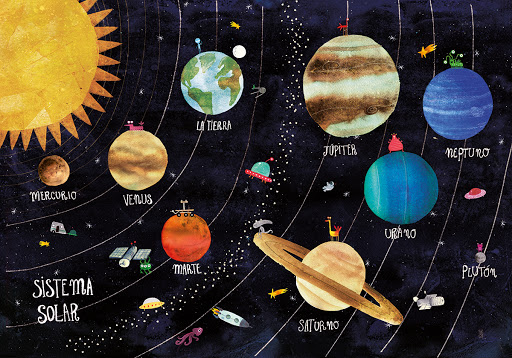
\includegraphics[height=2.0in,width=2.0in]{galaxia.jpg}
            \end{columns}
		\end{frame}
%%%Diapositiva
	\subsection{Matemáticas}	
	    \begin{frame}{Matemáticas}
			\justifying
			Las matemáticas juegan un papele muy importante, dentro del estudio del espacio, las galaxias, los sistemas, los planetas, etc.En sí, en todo el contenido del espacio. Tal es el caso de los movimientos de los palentes, sus rotaciones, etc. Un ejemplo es el cálculo del movimiento rotativo de la tierra, que viene dado por la siguiente fórmula:
            \begin{block}{Movimiento rotativo}
                En una \textcolor{red}{rotación} en un ángulo infinitesimal $\delta \theta$, se puede tomar $cos \delta \theta = 1$ y $sen \delta \theta = \delta \theta$, de modo que la expresión de la rotación plana pasa a ser:
                \textcolor{red}{${\displaystyle \mathbf {r} '=\mathbf {r} +\delta \theta (\mathbf {u} \times \mathbf {r} )}$}
            \end{block}
    	\end{frame}
    \section{Conclusiones}
        \begin{frame}{Conclusiones}
        Es importante leer y dar continuidad a los avancces cientificos de este ámbito, ya que sus estudios permiten hacer descubrimientos relevantes a nuestra vida en la Tierra y puede que, alguno de nosotros encuentre un punto focal interesante.
        \end{frame}
%%Diapositiva exclusiva para las referencias 
    \section{Referencias}
        \begin{frame}{Referencias}
            \begin{thebibliography}{10}
            	\bibitem{Author1990}
            	Equipo de Expertos\\
            	\newblock{\em El Sistema Solar y sus Planetas}.\\
            	Universidad Internacional de Valencia\\
            	\url{https://www.universidadviu.com/el-sistema-solar-y-sus-planetas/}
            	\bibitem{Author1990}
            	Kristen Erickson \\
            	\newblock{\em ¿Qué es una galaxia?}.\\
            	NASA Space Place\\
            	\url{https://spaceplace.nasa.gov/galaxy/sp/}
            	\bibitem{Author1990}
            	GeoEnciclopedia \\
            	\newblock{\em El Sistema Solar}.\\
            	\url{https://www.geoenciclopedia.com/sistema-solar/}
            	
            \end{thebibliography}
    \end{frame}
\end{document}